\documentclass{mcmthesis}
\mcmsetup{CTeX = true,   % 使用 CTeX 套装时,设置为 true
        tcn = 0000, problem = C,% 队伍控制号码,接受一个字符串作为值;选题,接受一个字符串作为值;
        sheet = true, %为真时将输出摘要页,否则不输出;默认为 true。
        color = red,  %设置控制页的题目号的颜色
        titleinsheet = true, %为真时将在摘要页输出标题,否则不输出;默认为 false。
        keywordsinsheet = true,%为真时将在摘要页输出关键字,否则不输出;默认为 false。
        titlepage = false,%为真时将输出标题页,否则不输出;默认为 true。
        abstract = true}%为真时将在标题页输出摘要和关键词,否则不输出;默认值为 true。
\usepackage{palatino}  %控制正文字体,若是不喜欢可以注释掉。
\usepackage{lipsum}
\usepackage{indentfirst}
\setlength{\parindent}{2em}
\title{The \LaTeX{} Template for MCM Version \MCMversion}
\author{\url{http://www.latexstudio.net}\\[3pt]  \href{http://www.latexstudio.net/}
  {
\includegraphics[width=7cm]{mcmthesis-logo}}}
\date{\today}

\makeatletter
\renewcommand*\l@section{\@dottedtocline{1}{12pt}{12pt}}
\makeatother

\begin{document}
\begin{abstract}
	The Abstract should be
	structured to include the following details: Background,
	the context and purpose of the study; Results, the main
	findings; Conclusions, brief summary and potential im-
	plications. Please minimize the use of abbreviations and
	do not cite references in the abstract.
	\begin{keywords}
		keyword1; keyword2
	\end{keywords}
\end{abstract}

\maketitle

\tableofcontents
\newpage

\section{Introduction}
	\subsection{Problem Background}
		\par As narcotic analgesics, opioids are primarily used for pain relief and anesthesia to reduce patients' suffering, which contribute a lot to modern medicine since its appearance. However, it also has many side effects, including itchiness, nausea, respiratory depression, constipation, and, what counts most, addiction. Considering the adverse effects above, we tend to enforce the regulation of opioids to reduce the risk of addiction.
		
		Nowadays, The United States is undergoing one of its worst drug crises caused by opioids. Hundreds of people die from opioid-related overdoses while more and more Americans are suffering from opioid addiction. The crisis has reached such a scale that, beyond the risks it brings to public health, the loss of people with advanced degrees will curb the development of economy and national security.
		
		With the data offered by Drug Enforcement Administration's Office of Diversion Control about the situation of drug abusing in five states, we can know more about the characteristics of opioid epidemic and find out the factors contributing to the growth in opioid use and addiction, so that we can set a therapy to alleviate the problem.


	\subsection{View of Our Work}
		\par For the first Problem, to describe the spread of opioids disorder, we manage to calculate the weight of each county with geographic information and drug cases, and we can adjust the weights with fully connected neural network. Then we build a LSTM(Long Short-Term Memory) Neural Network , which attempts to model time or sequence dependent behaviour, in order to predict multiple output time series based on multiple input time series, so that we can predict the number o/f drug case in all the counties next year.
		\par By comparing the predicted data and the data before, we can clearly find which place in all counties has the tendency to increase and view these counties as specific concerns. We found that the drug abuse cases tend to increase in the counties which are historically trapped in opioids overdose.		
		\par For the second problem, we need to take the census data into consideration. So we make a new input branch for our model to obtain the influence of social-economy influence. The new branch consists of three autoencoder layers, the output of the autoencoder will be put into merge layer, where the model can capture the most salient features of the training data.	
		\par Finally, we can analyze comprehensively to create a strategy to help governments counter the opioids crisis.
	\subsection{Assumptions}

		\par Due to the limited data of the pentential drug abuse cases, and other soc........,we use the
		following assumptions to complete our model. These simplified assumptions will be used through our paper and can be improved with more reliable data:
		\begin{itemize}
			\item The count of drug abuse cases in a county can be regared as a presentation of the total drug abuse cases in this county.
			\item The total drug abuse cases in a county is proportional to the count data we get. This is reasonable because ..................
			\item Neglect the diffierence of opioid medicine on kind, we view all the instance of opioid as one to our model.
		\end{itemize}
\begin{tabular}{cp{0.6\textwidth}}
	\toprule
	 Symbols & Description\\
	\midrule
	 $x$ & position \\
	 $v$ & velocity \\
	 $a$ & acceleration \\
	 $t$ & time \\
	 $F$ & force\\
	\bottomrule
\end{tabular}


$$
W_{i,j} = -a \cdot exp(\frac{(x_{i_{geo}} - x_{j_{geo}})^{2} + (y_{i_{geo}} - y_{j_{geo}})^{2}}{2c^{2}})
$$




\section{Analysis of the Problem}
\begin{figure}[h]
\small
\centering
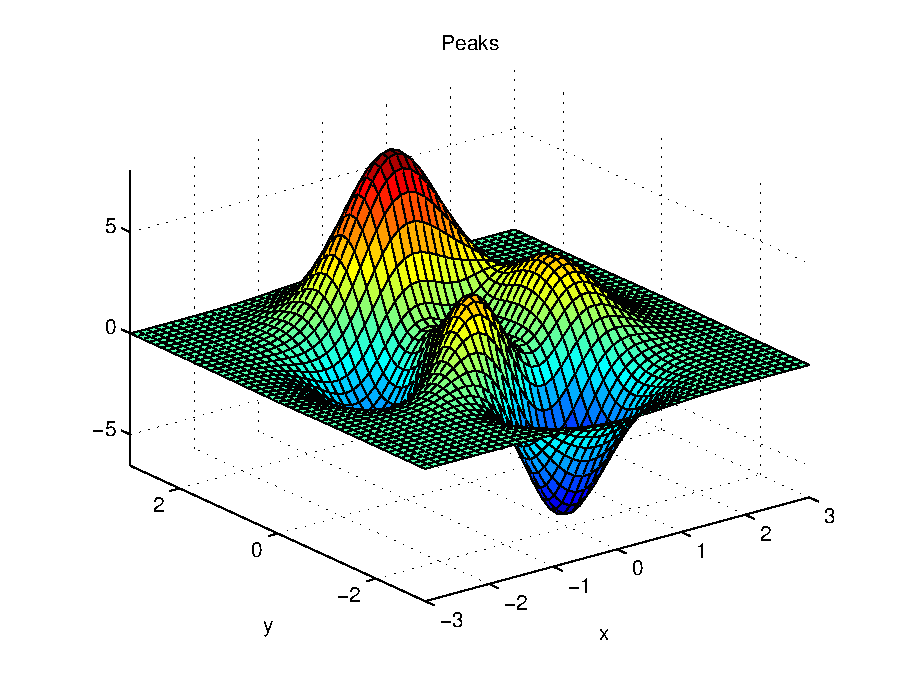
\includegraphics[width=12cm]{mcmthesis-aaa.eps}
\caption{aa} \label{fig:aa}
\end{figure}

\lipsum[8] \eqref{aa}
\begin{equation}
a^2 \label{aa}
\end{equation}

\[
  \begin{pmatrix}{*{20}c}
  {a_{11} } & {a_{12} } & {a_{13} }  \\
  {a_{21} } & {a_{22} } & {a_{23} }  \\
  {a_{31} } & {a_{32} } & {a_{33} }  \\
  \end{pmatrix}
  = \frac{{Opposite}}{{Hypotenuse}}\cos ^{ - 1} \theta \arcsin \theta
\]
\lipsum[9]

\[
  p_{j}=\begin{cases} 0,&\text{if $j$ is odd}\\
  r!\,(-1)^{j/2},&\text{if $j$ is even}
  \end{cases}
\]

\lipsum[10]

\[
  \arcsin \theta  =
  \mathop{{\int\!\!\!\!\!\int\!\!\!\!\!\int}\mkern-31.2mu
  \bigodot}\limits_\varphi
  {\mathop {\lim }\limits_{x \to \infty } \frac{{n!}}{{r!\left( {n - r}
  \right)!}}} \eqno (1)
\]

\section{Calculating and Simplifying the Model  }
\lipsum[11]

\section{The Model Results}
\lipsum[6]

\section{Validating the Model}
\lipsum[9]

\section{Conclusions}
\lipsum[6]

\section{A Summary}
\lipsum[6]

\section{Evaluate of the Mode}

\section{Strengths and weaknesses}
\lipsum[12]

\subsection{Strengths}
\begin{itemize}
\item \textbf{Applies widely}\\
This  system can be used for many types of airplanes, and it also
solves the interference during  the procedure of the boarding
airplane,as described above we can get to the  optimization
boarding time.We also know that all the service is automate.
\item \textbf{Improve the quality of the airport service}\\
Balancing the cost of the cost and the benefit, it will bring in
more convenient  for airport and passengers.It also saves many
human resources for the airline. \item \textbf{}
\end{itemize}

\begin{thebibliography}{99}
\bibitem{1} D.~E. KNUTH   The \TeX{}book  the American
Mathematical Society and Addison-Wesley
Publishing Company , 1984-1986.
\bibitem{2}Lamport, Leslie,  \LaTeX{}: `` A Document Preparation System '',
Addison-Wesley Publishing Company, 1986.
\bibitem{3}\url{http://www.latexstudio.net/}
\bibitem{4}\url{http://www.chinatex.org/}
\end{thebibliography}

\newpage
\section{References}
[1] Birnbaum, H. G., White, A. G., Schiller, M., Waldman, T., Cleveland, J. M., Roland, C. L. (2011). Societal costs of prescription opioid abuse, dependence, and misuse in the United States. Pain medicine, 12(4), 657-667.

[2] Han, B., Compton, W. M., Jones, C. M., Cai, R. (2015). Nonmedical prescription opioid use and use disorders among adults aged 18 through 64 years in the United States, 2003-2013. Jama, 314(14), 1468-1478.

[3] Che, Z., Sauver, J. S., Liu, H., Liu, Y. (2017). Deep Learning Solutions for Classifying Patients on Opioid Use. In AMIA Annual Symposium Proceedings (Vol. 2017, p. 525). American Medical Informatics Association.

[4] Kolodny, A., Courtwright, D. T., Hwang, C. S., Kreiner, P., Eadie, J. L., Clark, T. W., Alexander, G. C. (2015). The prescription opioid and heroin crisis: a public health approach to an epidemic of addiction. Annual review of public health, 36, 559-574.

[5] Walley, A. Y., Xuan, Z., Hackman, H. H., Quinn, E., Doe-Simkins, M., Sorensen-Alawad, A., ... Ozonoff, A. (2013). Opioid overdose rates and implementation of overdose education and nasal naloxone distribution in Massachusetts: interrupted time series analysis. Bmj, 346, f174.

[6] Cochran, B. N., Flentje, A., Heck, N. C., Van Den Bos, J., Perlman, D., Torres, J., ... Carter, J. (2014). Factors predicting development of opioid use disorders among individuals who receive an initial opioid prescription: mathematical modeling using a database of commercially-insured individuals. Drug and alcohol dependence, 138, 202-208.

[7] Duarte, R. V., Raphael, J. H., Haque, M. S., Southall, J. L., Ashford, R. L. (2012). A predictive model for intrathecal opioid dose escalation for chronic non-cancer pain. Pain Physician, 15(5), 363-369.

[8] Degenhardt, L., Charlson, F., Mathers, B., Hall, W. D., Flaxman, A. D., Johns, N., Vos, T. (2014). The global epidemiology and burden of opioid dependence: results from the global burden of disease 2010 study. Addiction, 109(8), 1320-1333.

[9] Fischer, B., Rehm, J., Tyndall, M. (2016). Effective Canadian policy to reduce harms from prescription opioids: learning from past failures. CMAJ, 188(17-18), 1240-1244.

[10] ELDesoky, E. S. (2007). Pharmacokinetic-pharmacodynamic crisis in the elderly. American journal of therapeutics, 14(5), 488-498.

[11] Fischer, B., Russell, C., Murphy, Y., Kurdyak, P. (2015). Prescription opioids, abuse and public health in Canada: is fentanyl the new centre of the opioid crisis?. Pharmacoepidemiology and drug safety, 24(12), 1334-1336.

[12] Ford, J. A., Schroeder, R. D. (2008). Academic strain and non-medical use of prescription stimulants among college students. Deviant Behavior, 30(1), 26-53.

[13] Makary, M. A., Overton, H. N., Wang, P. (2017). Overprescribing is major contributor to opioid crisis. BMJ: British Medical Journal (Online), 359.

[14] Rose, M. E. (2017). Are prescription opioids driving the opioid crisis? Assumptions vs facts. Pain Medicine, 19(4), 793-807.

[15] Manchikanti, L., Sanapati, J., Benyamin, R. M., Atluri, S., Kaye, A. D., Hirsch, J. A. (2018). Reframing the prevention strategies of the opioid crisis: focusing on prescription opioids, fentanyl, and heroin epidemic. Pain physician, 21(4), 309-326.

[16] Rummans, T. A., Burton, M. C.,  Dawson, N. L. (2018, March). How good intentions contributed to bad outcomes: the opioid crisis. In Mayo Clinic Proceedings (Vol. 93, No. 3, pp. 344-350). Elsevier.

[17] Hassanpour, S., Tomita, N., DeLise, T., Crosier, B.,  Marsch, L. A. (2018). Identifying substance use risk based on deep neural networks and Instagram social media data. Neuropsychopharmacology, 1.

[18] Weatherburn, D., Jones, C., Freeman, K., Makkai, T. (2003). Supply control and harm reduction: lessons from the Australian heroin ‘drought’. Addiction, 98(1), 83-91.

[19] Weiner, S. G., Malek, S. K., Price, C. N. (2017). The opioid crisis and its consequences. Transplantation, 101(4), 678-681.

\newpage



\begin{appendices}


\newpage
\section{First appendix}

\lipsum[13]

Here are simulation programmes we used in our model as follow.\\

\textbf{\textcolor[rgb]{0.98,0.00,0.00}{Input matlab source:}}
\lstinputlisting[language=Matlab]{./code/mcmthesis-matlab1.m}

\section{Second appendix}

some more text \textcolor[rgb]{0.98,0.00,0.00}{\textbf{Input C++ source:}}
\lstinputlisting[language=C++]{./code/mcmthesis-sudoku.cpp}

\end{appendices}
\end{document}

%%
%% This work consists of these files mcmthesis.dtx,
%%                                   figures/ and
%%                                   code/,
%% and the derived files             mcmthesis.cls,
%%                                   mcmthesis-demo.tex,
%%                                   README,
%%                                   LICENSE,
%%                                   mcmthesis.pdf and
%%                                   mcmthesis-demo.pdf.
%%
%% End of file `mcmthesis-demo.tex'.
